
\section{\label{sec:fixedptOrder}Orde Kekonvergenan untuk Iterasi Titik Tetap
\index{metode iterasi titik tetap!analisis}}

Misalkan $f$ adalah fungsi dengan titik tetap $\hat{x}$ dan $f'(\hat{x})$
ada. Misalkan $x_{0},x_{1},x_{2},\ldots$ merupakan barisan yang diperoleh
dari iterasi titik tetap ($x_{k+1}=f(x_{k})$ untuk semua $k\geq1$)
sedemikian sehingga ${\displaystyle \lim_{k\to\infty}x_{k}=\hat{x}}$
dan $x_{k}\neq\hat{x}$ untuk semua $k=0,1,2,\ldots$. Maka
\[
\frac{\left|x_{n+1}-\hat{x}\right|}{\left|x_{n}-\hat{x}\right|^{1}}=\left|\frac{f(x_{n})-f(\hat{x})}{x_{n}-\hat{x}}\right|
\]
dan
\begin{equation}
\lim_{n\to\infty}\left|\frac{f(x_{n})-f(\hat{x})}{x_{n}-\hat{x}}\right|=|f'(\hat{x})|.\label{eq:fixedPtOrder}
\end{equation}
Oleh karena itu, iterasi titik tetap konvergen secara linear selama
$f'(\hat{x})\neq0$. Proposisi berikut dapat disajikan sebagai korolari
dari Teorema Kekonvergenan Titik Tetap karena sebagian besar argumennya
sekadar mengulangi hal yang telah dikemukakan di sana, tetapi kita
memilih menyajikannya sebagai pernyataan terpisah berdasarkan persamaan
\ref{eq:fixedPtOrder}. Lebih tepatnya, kita memperoleh hasil berikut.
\begin{prop}
\label{prop:fixedPointErrorBound}(Batas Galat Titik Tetap) \index{Teorema!Batas Galat Titik Tetap}
Misalkan $f$ adalah fungsi terdiferensialkan dengan titik tetap $\hat{x}$
dan misalkan $[a,b]$ merupakan interval yang memuat $\hat{x}$. Jika
$|f'(x)|\leq M<1$ untuk semua $x\in[a,b]$ dan $f([a,b])\subseteq[a,b]$,
maka untuk sembarang nilai awal $x_{0}\in[a,b]$, iterasi titik tetap,
dengan $x_{k+1}=f(x_{k})$ untuk semua $k\geq0$, memberikan hampiran
bagi $\hat{x}$ dengan galat absolut tidak lebih dari $M^{k}|x_{0}-\hat{x}|$.
\end{prop}

\begin{proof}
Bukti induksi elementer (yang diminta dalam latihan) akan menunjukkan
bahwa $x_{k}\in[a,b]$ untuk semua $k\geq0$. Selanjutnya kita buktikan
batas galat tersebut. Galat absolut ketika menghampiri $\hat{x}$
dengan $x_{0}$ adalah $|x_{0}-\hat{x}|=M^{0}|x_{0}-\hat{x}|$ sehingga
pernyataan tersebut benar untuk $k=0$. Sekarang misalkan pernyataan
itu benar untuk suatu nilai tertentu tetapi sembarang $k\geq0$. Berdasarkan
teorema nilai rata-rata, terdapat $c$ dalam interval antara $\hat{x}$
dan $x_{k}$ sedemikian sehingga $f'(c)=\frac{f(x_{k})-f(\hat{x})}{x_{k}-\hat{x}}$.
Karena $\hat{x}$ dan $x_{k}$ keduanya berada di $[a,b]$, demikian
pula $c$. Akibatnya, $|f'(c)|\leq M$, sehingga $|f(x_{k})-f(\hat{x})|\leq M|x_{k}-\hat{x}|$.
Namun, $\hat{x}$ adalah titik tetap dari $f$, sehingga $f(\hat{x})=\hat{x}$,
dari sini diperoleh $|f(x_{k})-\hat{x}|\leq M|x_{k}-\hat{x}|$, dan
oleh karena itu $|x_{k+1}-\hat{x}|\leq M|x_{k}-\hat{x}|$. Berdasarkan
hipotesis induksi, $|x_{k}-\hat{x}|\leq M^{k}|x_{0}-\hat{x}|$, sehingga
$|x_{k+1}-\hat{x}|\leq M\cdot M^{k}|x_{0}-\hat{x}|=M^{k+1}|x_{0}-\hat{x}|$.
\end{proof}
Ketika $f'(\hat{x})=0$, persamaan \ref{eq:fixedPtOrder} menunjukkan
bahwa iterasi titik tetap tidak konvergen secara linear. Untuk setiap
barisan $\langle p_{n}\rangle$ yang konvergen ke $p$, jika $\lim_{n\to\infty}\frac{|p_{n+1}-p|}{|p_{n}-p|}=0$
kita mengatakan bahwa barisan tersebut konvergen secara superlinear
\index{kekonvergenan!superlinear} atau bahwa kekonvergenannya lebih
cepat daripada linear.

Perhatikan fungsi $f(x)=\frac{1}{8}x^{3}-x^{2}+2x+1$ dan $f_{1}(x)=-x^{3}+5x^{2}-3x-6$
dari bagian \ref{sec:Fixedpt}. Ingat bahwa $2$ adalah titik tetap
dari $f$ dan $3$ adalah titik tetap dari $f_{1}$ serta perhatikan
bahwa $f'(2)=\frac{3}{8}\cdot2^{2}-2\cdot2+2=-\frac{1}{2}$ dan $f_{1}'(3)=-3\cdot3^{2}+10\cdot3-3=0$
Akibatnya, kita mengharapkan iterasi titik tetap untuk $f_{1}$ konvergen
ke 3 lebih cepat daripada iterasi $f$ konvergen ke 2. Dengan $s_{0},s_{1},s_{2},\ldots=1.75,f(1.75),f(f(1.75)),\ldots$
dan $t_{0},t_{1},t_{2},\ldots=2.75,f_{1}(2.75),f_{1}(f_{1}(2.75)),\ldots$,
tabel \ref{tab:fixedPointOrderComparison} 
\begin{table}[h]
\hrule \caption{\label{tab:fixedPointOrderComparison}Membandingkan orde kekonvergenan
iterasi titik tetap ketika turunan pada titik tetap tidak nol ($s_{n}$)
dengan ketika turunan pada titik tetap bernilai nol ($t_{n}$).}

\centering{}\medskip{}
\begin{tabular}{c|cc}
$n$ & $|2-s_{n}|$ & $|3-t_{n}|$\tabularnewline
\hline 
0 & $2.5(10)^{-1}$ & $2.5(10)^{-1}$\tabularnewline
1 & $1.074(10)^{-1}$ & $2.343(10)^{-1}$\tabularnewline
2 & $5.644(10)^{-2}$ & $2.068(10)^{-1}$\tabularnewline
3 & $2.740(10)^{-2}$ & $1.623(10)^{-1}$\tabularnewline
4 & $1.388(10)^{-2}$ & $1.010(10)^{-1}$\tabularnewline
5 & $6.894(10)^{-3}$ & $3.984(10)^{-2}$\tabularnewline
6 & $3.459(10)^{-3}$ & $6.286(10)^{-3}$\tabularnewline
7 & $1.726(10)^{-3}$ & $1.578(10)^{-4}$\tabularnewline
8 & $8.640(10)^{-4}$ & $9.966(10)^{-8}$\tabularnewline
9 & $4.318(10)^{-4}$ & $3.973(10)^{-14}$\tabularnewline
10 & $2.159(10)^{-4}$ & $6.317(10)^{-27}$\tabularnewline
\end{tabular}\medskip{}
\hrule 
\end{table}
menunjukkan perbandingan laju kekonvergenannya. $\langle s_{n}\rangle$
konvergen secara linear seperti yang diharapkan, sedangkan $\langle t_{n}\rangle$
tampaknya konvergen secara kuadratik. Empat eksponen terakhir pada
kolom $|3-t_{n}|$ adalah $-4,-8,-14,-27$, yang menunjukkan bahwa
banyaknya angka signifikan dalam akurasi kira-kira berlipat dua pada
setiap iterasi. Dengan kata lain, galat suatu suku kira-kira merupakan
kuadrat galat suku sebelumnya (artinya $\alpha=2$ dalam definisi
orde kekonvergenan).

\label{FixedPointIterationConvergesQuadratically}Teorema Taylor akan
memberikan bukti yang kita perlukan bahwa kekonvergenan ini memang
kuadratik. Misalkan $f$ memiliki turunan ketiga dalam suatu lingkungan
$\hat{x}$. Definisikan $e_{n}=\hat{x}-x_{n}$. Maka, menurut teorema
Taylor, $\hat{x}=f(\hat{x})=f(x_{n}+e_{n})=f(x_{n})+e_{n}f'(x_{n})+\frac{1}{2}e_{n}^{2}f''(x_{n})+O(e_{n}^{3})$.
Namun, $f(x_{n})=x_{n+1}$ sehingga kita peroleh
\begin{equation}
\hat{x}-x_{n+1}=e_{n+1}=e_{n}f'(x_{n})+\frac{1}{2}e_{n}^{2}f''(x_{n})+O(e_{n}^{3}).\label{eq:fixedptIsQuadratic1}
\end{equation}
Juga menurut teorema Taylor, $f'(\hat{x})=f'(x_{n}+e_{n})=f'(x_{n})+e_{n}f''(x_{n})+O(e_{n}^{2})$.
Namun, $f'(\hat{x})=0$ sehingga
\begin{equation}
f'(x_{n})=-e_{n}f''(x_{n})-O(e_{n}^{2}).\label{eq:fixedptIsQuadratic2}
\end{equation}
Dengan menyubstitusikan \ref{eq:fixedptIsQuadratic2} ke dalam \ref{eq:fixedptIsQuadratic1},
\begin{eqnarray*}
e_{n+1} & = & e_{n}(-e_{n}f''(x_{n})-O(e_{n}^{2}))+\frac{1}{2}e_{n}^{2}f''(x_{n})+O(e_{n}^{3})\\
 & = & -\frac{1}{2}e_{n}^{2}f''(x_{n})+O(e_{n}^{3}).
\end{eqnarray*}
Jadi, $\frac{\hat{x}-x_{n+1}}{(\hat{x}-x_{n})^{2}}=\frac{e_{n+1}}{e_{n}^{2}}=-\frac{1}{2}f''(x_{n})+O(e_{n})$
dan
\[
\lim_{n\to\infty}\frac{|\hat{x}-x_{n+1}|}{|\hat{x}-x_{n}|^{2}}=\lim_{n\to\infty}\left|\frac{1}{2}f''(x_{n})+O(e_{n})\right|=\left|\frac{1}{2}f''(\hat{x})\right|,
\]
yang menunjukkan bahwa kekonvergenannya setidaknya kuadratik. Jika
$f''(\hat{x})$ kebetulan bernilai 0, kekonvergenannya menjadi superkuadratik.

Ringkasnya, jika secara kebetulan pada suatu titik tetap $\hat{x}$,
$f'(\hat{x})=0$, iterasi titik tetap berhasil dan cepat untuk nilai
awal di dekat $\hat{x}$. Namun, ketika $f'(\hat{x})\neq0$, iterasi
titik tetap mungkin gagal konvergen ke $\hat{x}$, dan ketika konvergen,
kekonvergenannya lambat. Akan tetapi, ada perbaikan cepat (cepat diterapkan,
bukan cepat dijelaskan) untuk sebagian kekurangan ini ketika $f'(\hat{x})\neq0$.
Pertama-tama, kita akan berfokus pada kecepatan kekonvergenan.

Misalkan barisan $\langle c_{n}\rangle$ didefinisikan oleh
\begin{eqnarray*}
c_{0} & = & 1\\
c_{k} & = & \cos(c_{k-1}),\quad k>0.
\end{eqnarray*}
Anda seharusnya dapat memverifikasi bahwa beberapa suku pertama barisan
ini adalah (secara hampiran)
\[
1,.5403,.8575,.6542,.7934,\ldots
\]
Ini tepat merupakan barisan yang Anda buat dalam eksperimen kalkulator
\vpageref{sec:Fixedpt} pada bagian \ref{sec:Fixedpt}. Definisikan
barisan baru $\langle a_{n}\rangle$ dengan
\[
a_{n}=c_{n}-\frac{(c_{n+1}-c_{n})^{2}}{c_{n+2}-2c_{n+1}+c_{n}}.
\]
Tabel \ref{tab:deltaSquaredAcceleration} 
\begin{table}
\hrule 

\caption{\label{tab:deltaSquaredAcceleration}Mempercepat kekonvergenan suatu
barisan yang konvergen secara linear.}

\centering{}\medskip{}
\begin{tabular}{c|cccccc}
$n$ & $c_{n}$ & $a_{n}$ & $|c_{n}-c|$ & $|a_{n}-c|$ & $\left|\frac{a_{n}-c}{c_{n}-c}\right|$ & $\frac{\left|a_{n+1}-c\right|}{\left|a_{n}-c\right|^{2}}$\tabularnewline
\hline 
0 & 1 & $.728010$ & $2.609(10)^{-1}$ & $1.107(10)^{-2}$ & $.0934$ & $.0110$\tabularnewline
1 & $.5403$ & $.733665$ & $1.987(10)^{-1}$ & $5.419(10)^{-3}$ & $.0639$ & $44.19$\tabularnewline
2 & $.8575$ & $.736906$ & $1.184(10)^{-1}$ & $2.178(10)^{-3}$ & $.0400$ & $74.17$\tabularnewline
3 & $.6542$ & $.738050$ & $8.479(10)^{-2}$ & $1.034(10)^{-3}$ & $.0274$ & $217.9$\tabularnewline
4 & $.7934$ & $.738636$ & $5.439(10)^{-2}$ & $4.490(10)^{-4}$ & $.0180$ & $419.4$\tabularnewline
5 & $.7103$ & $.738876$ & $3.771(10)^{-2}$ & $2.085(10)^{-4}$ & $.0122$ & $1034$\tabularnewline
6 & $.7639$ & $.738992$ & $2.487(10)^{-2}$ & $9.289(10)^{-5}$ & $.0081$ & \tabularnewline
7 & $.7221$ &  &  &  &  & \tabularnewline
8 & $.7504$ &  &  &  &  & \tabularnewline
\end{tabular}\medskip{}
\hrule 
\end{table}
 menunjukkan beberapa suku pertama kedua barisan beserta sejumlah
analisis galat. Seperti yang dijanjikan, barisan $\langle a_{n}\rangle$
konvergen lebih cepat daripada $\langle c_{n}\rangle$, sebagaimana
ditunjukkan oleh fakta bahwa $\left|\frac{a_{n}-c}{c_{n}-c}\right|$
menuju nol. Namun, kolom terakhir tabel menunjukkan bahwa kekonvergenan
$\langle a_{n}\rangle$ ke $c$ bukan kuadratik.

Secara lebih umum, misalkan $\langle p_{n}\rangle$ adalah sembarang
barisan yang konvergen secara linear ke $p$. Maka kita memiliki ${\displaystyle \lim_{n\to\infty}}\frac{|p-p_{n+1}|}{|p-p_{n}|}=\lambda\neq0$,
sehingga kita mengharapkan $\frac{|p-p_{n+2}|}{|p-p_{n+1}|}\approx\frac{|p-p_{n+1}|}{|p-p_{n}|}\approx\lambda$
untuk $n$yang cukup besar, dan dari sini kita peroleh $|(p-p_{n+2})(p-p_{n})|\approx|p-p_{n+1}|^{2}$.
Dengan mengasumsikan bahwa $p-p_{n+2}$ dan $p-p_{n}$ bertanda sama
untuk $n$\footnote{Hal ini akan terjadi dalam dua keadaan yang umum: semua $\hat{x}-x_{n}$
bertanda sama, atau tanda $\hat{x}-x_{n}$ berselang-seling. Jadi,
asumsi ini bukanlah asumsi yang tidak masuk akal.}, kita dapat menghapus nilai mutlak dan memperoleh
\begin{eqnarray*}
(p-p_{n+2})(p-p_{n}) & \approx & (p-p_{n+1}){}^{2}\\
p^{2}-(p_{n+2}+p_{n})p+p_{n+2}p_{n} & \approx & p^{2}-2p_{n+1}p+p_{n+1}^{2}\\
(-p_{n+2}+2p_{n+1}-p_{n})p & \approx & -p_{n+2}p_{n}+p_{n+1}^{2}\\
p & \approx & \frac{p_{n+2}p_{n}-p_{n+1}^{2}}{p_{n+2}-2p_{n+1}+p_{n}}.
\end{eqnarray*}
Oleh karena itu, kita dapat mengambil sembarang tiga suku berurutan
dari $\langle p_{n}\rangle$ dan memperkirakan $p$ menggunakan rumus
ini. Untuk $n$yang cukup besar, perkiraan ini akan menjadi hampiran
yang jauh lebih baik bagi $p$ daripada $p_{n}$. Namun, sebagaimana
kita dapat menyatakan $|(p-p_{n+2})(p-p_{n})|\approx|p-p_{n+1}|^{2}$,
harus pula berlaku $p_{n+2}p_{n}\approx p_{n+1}^{2}$, sehingga pembilang
hampiran kita mendekati nol. Tentu saja, itu berarti penyebutnya juga
harus mendekati nol, sebab hasil baginya adalah $p$, suatu nilai
yang mungkin tidak nol. Untuk menghindari sebagian galat yang melekat
dalam perhitungan ini, sebaiknya kita menghitung hampiran yang ekuivalen
secara aljabar \index{metode delta-kuadrat Aitken}\index{metode!delta-kuadrat Aitken|see{metode delta-kuadrat Aitken}}
\begin{equation}
p\approx p_{n}-\frac{(p_{n+1}-p_{n})^{2}}{p_{n+2}-2p_{n+1}+p_{n}}\label{eq:aitkensDeltaSquared}
\end{equation}
 sebagai gantinya. Mari kembali meninjau barisan $\langle s_{n}\rangle$
dan menerapkan hampiran ini.

Definisikan $a_{n}=s_{n}-\frac{(s_{n+1}-s_{n})^{2}}{s_{n+2}-2s_{n+1}+s_{n}}$
dan perhatikan tabel 
\begin{table}[h]
\hrule \caption{\label{tab:fixedPointAitkens}Membandingkan iterasi titik tetap ketika
turunan pada titik tetap tidak nol, $s_{n}$, dengan barisan delta-kuadrat
Aitken, $a_{n}$.}

\centering{}\medskip{}
\begin{tabular}{c|ccccc}
$n$ & $s_{n}$ & $|2-s_{n}|$ & $a_{n}$ & $|2-a_{n}|$ & $\frac{|2-a_{n}|}{|2-s_{n+2}|^{2}}$\tabularnewline
\hline 
0 & $1.75$ & $2.5(10)^{-1}$ & $1.99506842493985$ & $4.931(10)^{-3}$ & $1.54$\tabularnewline
1 & $2.107421875$ & $1.074(10)^{-1}$ & $1.999022858310434$ & $9.771(10)^{-4}$ & $1.30$\tabularnewline
2 & $1.943559146486223$ & $5.644(10)^{-2}$ & $1.999737171760319$ & $2.628(10)^{-4}$ & $1.36$\tabularnewline
3 & $2.027401559734717$ & $2.740(10)^{-2}$ & $1.999937151202653$ & $6.284(10)^{-5}$ & $1.32$\tabularnewline
4 & $1.986114080555812$ & $1.388(10)^{-2}$ & $1.999983969455146$ & $1.603(10)^{-5}$ & $1.32$\tabularnewline
5 & $2.006894420349172$ & $6.894(10)^{-3}$ &  &  & \tabularnewline
6 & $1.996540947531514$ & $3.459(10)^{-3}$ &  &  & \tabularnewline
\end{tabular}\medskip{}
\hrule 
\end{table}
 \ref{tab:fixedPointAitkens} yang membandingkan kedua barisan $\langle s_{n}\rangle$
dan $\langle a_{n}\rangle$. $\langle a_{n}\rangle$ konvergen jauh
lebih cepat daripada barisan yang konvergen secara linear dan menjadi
asalnya, persis seperti sebelumnya! Fakta bahwa $\frac{|2-a_{n}|}{|2-s_{n}|^{2}}\approx1.32$
merupakan bukti bagi pernyataan ini, tetapi kekonvergenan $\langle a_{n}\rangle$
tetap linear. Anda dapat memeriksa bahwa rasio $\frac{|2-a_{n+1}|}{|2-a_{n}|^{1}}$
kira-kira konstan (sekitar $0.25$) untuk $n=0,1,2,3,4$. Pastikan
Anda memahami mengapa hal ini menyiratkan kekonvergenan linear dan
dapat menghitung sendiri $a_{n}$ dalam tabel ini sebelum melanjutkan
membaca.

Secara praktis, tidak ada gunanya menghitung semua suku $a_{0},a_{1},\ldots,a_{n-2}$
seperti yang dilakukan dalam tabel. Suku-suku $\langle a_{n}\rangle$
hanya bergantung pada suku-suku $\langle s_{n}\rangle$ , sehingga
$a_{n-2}$ tetap dapat dihitung tanpa terlebih dahulu menghitung $a_{0},a_{1},\ldots,a_{n-3}$.
Tabel menampilkan semuanya hanya untuk tujuan ilustrasi dan agar Anda
mendapat latihan menggunakan rumus \ref{eq:aitkensDeltaSquared}.
Hal penting yang perlu diperhatikan adalah bahwa $a_{n}$ memiliki
kira-kira dua kali lebih banyak angka signifikan yang akurat dibandingkan
$s_{n+2}$ (karena $|2-a_{n}|\approx|2-s_{n+2}|^{2}$). Akibatnya,
$a_{0}$ merupakan hampiran yang jauh lebih baik daripada $s_{2}$. 

\begin{digression}{Metode delta-kuadrat Aitken dirancang untuk sembarang barisan yang konvergen secara linear, bukan hanya barisan yang diperoleh dari iterasi titik tetap.}

\noindent Penurunan \ref{eq:aitkensDeltaSquared}, yang disebut rumus
delta-kuadrat Aitken, sama sekali tidak merujuk pada iterasi titik
tetap. Bahkan, penurunan tersebut tidak membuat asumsi apa pun tentang
asal barisannya. Asalnya tidak berpengaruh. Barisan itu dapat berupa
barisan jumlah parsial, barisan hasil kali parsial, barisan yang diperoleh
dari sembarang relasi rekurensi, barisan yang berasal dari teori bilangan,
atau apa pun yang lain. Satu-satunya karakteristik penting adalah
bahwa barisan tersebut konvergen dan melakukannya secara linear.

Deret $\frac{1}{1}-\frac{1}{3}+\frac{1}{5}-\frac{1}{7}+\frac{1}{9}-\cdots$
konvergen ke $\frac{\pi}{4}$ secara linear, sehingga metode delta-kuadrat
Aitken seharusnya membantu. Jika kita tetapkan $p_{n}=\sum_{k=1}^{n}\frac{(-1)^{k+1}}{2k-1}$
sebagai jumlah parsial ke- $n$ , maka $p_{2}=\frac{13}{15}$, $p_{3}=\frac{76}{105}$,
$p_{4}=\frac{263}{315}$, dan $p_{5}=\frac{2578}{3465}$. Ekstrapolasi
Aitken menghasilkan $a_{2}=\frac{13}{15}-\frac{(\frac{76}{105}-\frac{13}{15})^{2}}{\frac{263}{315}-2\frac{76}{105}+\frac{13}{15}}=\frac{1321}{1680}$
dan $a_{3}=\frac{76}{105}-\frac{(\frac{263}{315}-\frac{76}{105})^{2}}{\frac{2578}{3465}-2\frac{263}{315}+\frac{76}{105}}=\frac{989}{1260}$.
$\frac{|\frac{\pi}{4}-p_{4}|^{2}}{|\frac{\pi}{4}-a_{2}|}\approx2.6$
dan $\frac{|\frac{\pi}{4}-p_{5}|^{2}}{|\frac{\pi}{4}-a_{3}|}\approx3.5$
sehingga ekstrapolasi menghasilkan galat yang lebih kecil daripada
kuadrat galat pada barisan semula.

\end{digression}

Barangkali fakta ini memberi Anda suatu gagasan. Setelah $s_{2}$
dihitung, kita dapat menggunakan persamaan \ref{eq:aitkensDeltaSquared},
yang juga dikenal sebagai \index{metode delta-kuadrat Aitken}metode
delta-kuadrat Aitken, untuk menghitung hampiran yang lebih baik daripada
yang telah kita miliki. Setelah memperoleh hampiran yang baik ini,
rasanya agak konyol jika kita mengesampingkannya dan terus menghitung
$s_{3}=f(s_{2}),s_{4}=f(s_{3}),$ dan seterusnya. Bagaimana jika kita
menggunakan $a_{0}$ sebagai pengganti $s_{3}$ dalam iterasi? Dengan
kata lain, kita akan memperoleh $s_{1}=f(s_{0}),s_{2}=f(s_{1}),s_{3}=a_{0},s_{4}=f(s_{3}),$
dan seterusnya. Hal itu seharusnya memperbaiki $s_{3},s_{4},\mbox{ dan }s_{5}$.
Setelah memperoleh $s_{5}$ kita kembali memiliki tiga iterasi titik
tetap berurutan, sehingga dapat menerapkan metode delta-kuadrat Aitken
lagi. Alih-alih menghitung $s_{6}=f(s_{5})$, kita dapat memperoleh
hampiran yang semestinya lebih baik dengan menerapkan persamaan \ref{eq:aitkensDeltaSquared}
pada $s_{3},s_{4},\mbox{ dan }s_{5}$. Dengan kata lain, $s_{6}=a_{3}$,
$s_{7}=f(s_{6})$, $s_{8}=f(s_{7})$. Sekali lagi, kita memiliki tiga
iterasi titik tetap berurutan, sehingga $s_{9}=a_{6}$, dan seterusnya.
Ini menghasilkan barisan berikut

\begin{center}
\begin{tabular}{ccc}
$1.75,$ & $2.107421875,$ & $1.943559146486222,$\tabularnewline
$1.995068424939850,$ & $2.002459692429676,$ & $1.998768643123618,$\tabularnewline
$1.999997974970982,$ & $2.000001012513483,$ & $1.999999493743001,$\tabularnewline
$1.999999999999658,$ & $2.000000000000170,$ & $1.999999999999914,$\tabularnewline
$1.999999999999999,$ & $\ldots$ & \tabularnewline
\end{tabular}
\par\end{center}

\noindent yang konvergen ke 2 dengan sangat cepat dibandingkan $\langle s_{n}\rangle$.
Jika kita menganggap perhitungan $s_{1},s_{2},s_{4},s_{5},s_{7},s_{8},\ldots$
sebagai perhitungan perantara dan memusatkan perhatian pada subbarisan
$s_{0},s_{3},s_{6},s_{9},\ldots=s_{0},a_{0},a_{3},a_{6},\ldots$ sebagai
barisan tersendiri, kita memperoleh 
\[
1.75,\ 1.995068424939850,\ 1.999997974970982,\ 1.999999999999658,\ 1.999999999999999,\ldots
\]
yang konvergen dengan sangat cepat! Pembentukan subbarisan ini sebagai
barisan tersendiri disebut \index{metode Steffensen}\index{metode!Steffensen|see{metode Steffensen}}
metode Steffensen, dan kekonvergenannya kuadratik selama $\langle s_{n}\rangle$
konvergen. Berikut adalah argumen heuristik bahwa metode Steffensen
memberikan kekonvergenan kuadratik. Seperti terlihat, galat pada $s_{2}$
tidak jauh berbeda dari galat pada $s_{0}$. Namun, $a_{0}$ memiliki
galat yang kira-kira sama dengan kuadrat galat pada $s_{2}$, sehingga
galat pada $a_{0}$ kira-kira sama dengan kuadrat galat pada $s_{0}$.
Demikian pula, galat pada $s_{5}$ tidak jauh berbeda dari galat pada
$a_{0}=s_{3}$. Namun, galat pada $a_{1}$ kira-kira sama dengan kuadrat
galat pada $s_{5}$, sehingga galat pada $a_{1}$ kira-kira sama dengan
kuadrat galat pada $a_{0}$. Demikian pula, galat pada $a_{n+1}$
kira-kira sama dengan kuadrat galat pada $a_{n}$.

Dengan menerapkan metode Steffensen pada fungsi $f(x)=\cos x$ dengan
$x_{0}=1$, kita dapat mempercepat kekonvergenan barisan $\langle c_{n}\rangle$
secara drastis. Tabel \ref{tab:steffensens2} 
\begin{table}
\hrule 

\caption{\label{tab:steffensens2}Metode Steffensen diterapkan pada $f(x)=\cos x$.}
\medskip{}

\begin{centering}
\begin{tabular}{c|ccccc}
$n$ & $a_{n}$ & $g(a_{n})$ & $g(g(a_{n}))$ & $|a_{n}-c|$ & $\frac{\left|a_{n+1}-c\right|}{\left|a_{n}-c\right|^{2}}$\tabularnewline
\hline 
0 & 1 & $.5403023058681398$ & $.8575532158463934$ & $2.609(10)^{-1}$ & $.162$\tabularnewline
1 & $.7280103614676171$ & $.7464997560452203$ & $.7340702837365296$ & $1.107(10)^{-2}$ & $.148$\tabularnewline
2 & $.7390669669086738$ & $.7390973701357808$ & $.7390768902228948$ & $1.816(10)^{-5}$ & $.148$\tabularnewline
3 & $.7390851331660755$ & $.739085133248225$ & $.739085133192888$ & $4.908(10)^{-11}$ & $.148$\tabularnewline
4 & $.7390851332151607$ &  &  & $3.063(10)^{-17}$ & \tabularnewline
\end{tabular}
\par\end{centering}
\medskip{}
\hrule 
\end{table}
 menunjukkan beberapa suku pertama $\langle a_{n}\rangle$ beserta
sejumlah analisis galat. Kolom terakhir tabel menunjukkan bahwa 
\[
\lim_{n\to\infty}\frac{\left|a_{n+1}-c\right|}{\left|a_{n}-c\right|^{2}}\approx.148
\]
dan, akibatnya, barisan $\langle a_{n}\rangle$ konvergen secara kuadratik.

Terakhir, kita memiliki dua cara untuk memperoleh kekonvergenan cepat
dari iterasi titik tetap. Pertama, kita cukup melakukan iterasi ketika
turunan fungsi bernilai nol pada titik tetapnya. Kedua, kita menggunakan
metode Steffensen.

\subsection{Diagram Kekonvergenan\index{diagram kekonvergenan}}

Mempercepat iterasi titik tetap hanya mengatasi salah satu kekurangan
metode tersebut. Masih ada masalah divergensi dari titik tetap ketika
nilai mutlak turunan fungsi sama dengan atau lebih besar daripada
1. Metode Steffensen membantu. Bandingkan Gambar \ref{fig:FiveConvergenceDiagrams}
dengan Gambar \ref{fig:SixConvergenceDiagrams}. Diagram kekonvergenan
untuk metode Steffensen menunjukkan kekonvergenan pada interval nilai
awal yang lebih luas. Selain itu, untuk $f_{1}$ dan $f_{2}$ , metode
Steffensen menemukan ketiga titik tetap, sama seperti iterasi titik
tetap pada $f_{6}$ . 
\begin{figure}
\caption{\label{fig:FiveConvergenceDiagrams}Diagram kekonvergenan untuk 5
fungsi yang memiliki titik-titik tetap yang sama---metode Steffensen.}

\bigskip{}

\begin{centering}
$f_{1}$: 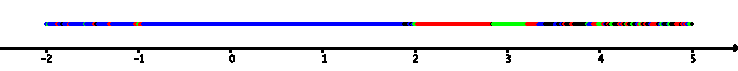
\includegraphics{figures/roots-order1}
\par\end{centering}
\begin{centering}
$f_{2}$: 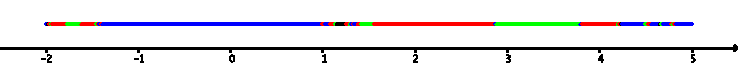
\includegraphics{figures/roots-order2}
\par\end{centering}
\begin{centering}
$f_{3}$: 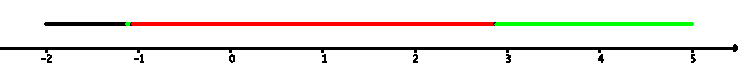
\includegraphics{figures/roots-order3}
\par\end{centering}
\begin{centering}
$f_{4}$: 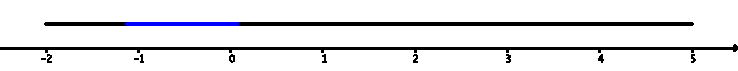
\includegraphics{figures/roots-order4}
\par\end{centering}
\begin{centering}
$f_{5}$: 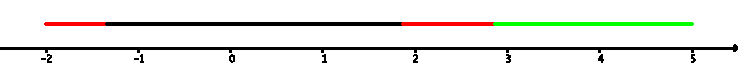
\includegraphics{figures/roots-order5}
\par\end{centering}
\centering{}hitam: tidak konvergen; hijau: konvergen ke $3$; merah:
konvergen ke $1+\sqrt{3}$; biru: konvergen ke $1-\sqrt{3}$
\end{figure}


\subsection{Metode Steffensen (kode semu)\index{metode Steffensen!kode semu}}

Karena metode Steffensen sangat rentan terhadap galat titik-mengambang,
kita melakukan pemeriksaan awal terhadap kekonvergenan sebelum langkah
delta-kuadrat Aitken. Hal ini membantu mencegah galat besar atau pembagian
dengan nol pada Langkah 4.

\begin{pseudocode} 
\begin{description}
\item [{Asumsi:}] Iterasi titik tetap konvergen ke suatu titik tetap dari
$f$ dengan nilai awal $x_{0}$.
\item [{Masukan:}] Nilai awal $x_{0}$; fungsi $f$; akurasi yang diinginkan
$tol$; jumlah maksimum iterasi $N$.
\item [{Langkah~1:}] Untuk $j=1\ldots N$ lakukan Langkah 2-6:

\begin{description}
\item [{Langkah~2:}] Tetapkan $x_{1}=f(x_{0})$; $x_{2}=f(x_{1})$
\item [{Langkah~3:}] Jika $|x_{2}-x_{1}|\leq tol$ maka kembalikan $x_{2}$
\item [{Langkah~4:}] Tetapkan $x=x_{0}-\frac{(x_{1}-x_{0})^{2}}{x_{2}-2x_{1}+x_{0}}$
\item [{Langkah~5:}] Jika $|x-x_{2}|\leq tol$ maka kembalikan $x$;
\item [{Langkah~6:}] Tetapkan $x_{0}=x$;
\end{description}
\item [{Langkah~7:}] Cetak ``Metode gagal. Jumlah iterasi maksimum terlampaui.''
\item [{Keluaran:}] Hampiran $x$ yang mendekati titik tetap eksak atau
pesan kegagalan.
\end{description}
\end{pseudocode}  

\subsection{Konsep Utama}
\begin{description}
\item [{Metode~delta-kuadrat~Aitken:}] Jika $\langle p_{n}\rangle$ konvergen
secara linear ke $p$, barisan $\langle a_{n}\rangle$ yang didefinisikan
oleh $a_{n}=p_{n}-\frac{(p_{n+1}-p_{n})^{2}}{p_{n+2}-2p_{n+1}+p_{n}}$
konvergen lebih cepat ke $p$, tetapi tetap berorde linear.
\item [{Batas~Galat~Titik~Tetap:}] \index{Teorema!Batas Galat Titik Tetap}
Misalkan $f$ adalah fungsi terdiferensial yang memiliki titik tetap
$\hat{x}$ dan misalkan $[a,b]$ adalah interval yang memuat $\hat{x}$.
 Jika $|f'(x)|\leq M<1$ untuk setiap $x\in[a,b]$ dan $f([a,b])\subseteq[a,b]$,
maka untuk sembarang nilai awal $x_{0}\in[a,b]$, iterasi titik tetap
dengan $x_{k+1}=f(x_{k})$ untuk setiap $k\geq0$ menghasilkan hampiran
terhadap $\hat{x}$ dengan galat absolut tidak lebih dari $M^{k}|x_{0}-\hat{x}|$.
\item [{Orde~Kekonvergenan~untuk~Iterasi~Titik~Tetap:}] Misalkan $f$
adalah fungsi dengan titik tetap $\hat{x}$ dan $f'(\hat{x})$ ada.
Misalkan $x_{0},x_{1},x_{2},\ldots$ merupakan barisan yang diperoleh
dari iterasi titik tetap ($x_{k+1}=f(x_{k})$ untuk setiap $k\geq1$)
sedemikian sehingga ${\displaystyle \lim_{k\to\infty}x_{k}=\hat{x}}$
dan $x_{k}\neq\hat{x}$ untuk setiap $k=0,1,2,\ldots$. Maka barisan
$\langle x_{n}\rangle$ konvergen secara linear ke $\hat{x}$ jika
$f'(\hat{x})\neq0$ dan berorde setidaknya kuadratik jika $f'(\hat{x})=0$.
\item [{Metode~Steffensen:}] \index{metode Steffensen}Modifikasi iterasi
titik tetap dengan setiap suku ketiga dihitung menggunakan metode
delta-kuadrat Aitken.
\item [{Kekonvergenan~superlinear:}] \index{kekonvergenan!superlinear}
Jika barisan $p_{0},p_{1},p_{2},\ldots$ konvergen ke $p$ dan ${\displaystyle \lim_{k\to\infty}\frac{|p_{k+1}-p|}{|p_{k}-p|}=0}$,
maka barisan tersebut dikatakan konvergen secara superlinear.
\item [{Kekonvergenan~superkuadratik:}] \index{kekonvergenan!superkuadratik}
Jika barisan $p_{0},p_{1},p_{2},\ldots$ konvergen ke $p$ dan ${\displaystyle \lim_{k\to\infty}\frac{|p_{k+1}-p|}{|p_{k}-p|^{2}}=0}$,
maka barisan tersebut dikatakan konvergen secara superkuadratik.
\end{description}

\subsection{Octave\label{subsec:WhileLoop}}

Pada Bagian \ref{sec:Speed}, kita telah mempelajari perulangan \texttt{for}.
Dengan perulangan \texttt{for}, Anda harus mengetahui berapa kali
perulangan itu hendak dijalankan, atau setidaknya menentukan jumlah
maksimum. Anda dapat menghentikan perulangan \texttt{for} sebelum
selesai dengan keluar (mengembalikan nilai) dari fungsi. Namun, adakalanya
Anda tidak tahu berapa kali perulangan perlu dijalankan dan bahkan
tidak memiliki batas maksimum yang sesuai. Dalam kasus ini, perulangan
\texttt{while} \index{Octave!perulangan while@perulangan \texttt{while}}
lebih tepat. Perulangan \texttt{while} akan terus berulang selama
kondisi tertentu terpenuhi; Anda sendiri yang menentukan kondisi tersebut.
Sintaks perulangan while adalah \begin{verbatim}
while (condition)
  do something. 
end%while
\end{verbatim}, tetapi harus digunakan dengan hati-hati. \texttt{for} selalu memiliki
akhir, tetapi perulangan \texttt{while} bisa tidak berakhir jika diprogram
dengan ceroboh. Jika \texttt{condition} pada perulangan \texttt{while}
tidak pernah terpenuhi, perulangan akan berjalan tanpa henti! Berikut
contoh sederhana perulangan \texttt{while} yang tidak pernah berakhir.
Jangan jalankan! \begin{verbatim}
i=0;
while (i<12)
  disp("Help! I'm stuck in a never-ending loop!!")
end%while
\end{verbatim} Masalahnya, \texttt{i} ditetapkan kurang dari 12 dan tidak pernah
berubah, sehingga selalu tetap kurang dari 12. Dengan demikian, kondisi
perulangan \texttt{while} ini selalu terpenuhi. Perulangan ini dapat
dengan mudah diubah agar berhenti. Jika kita menaikkan \texttt{i}
di dalam perulangan, perulangan tersebut akan berakhir. Modifikasi
terhadap perulangan tanpa akhir ini benar-benar berakhir dan menampilkan
pesan sebanyak 12 kali: \begin{verbatim}
i=0;
while (i<12)
  disp("That's better. I can handle a dozen iterations.")
  i=i+1;
end%while
\end{verbatim} Sebagai catatan, setiap perulangan \texttt{for} dapat digantikan
oleh perulangan \texttt{while} seperti yang satu ini. 

Kita adalah manusia. Tak terelakkan, suatu saat kita akan memprogram
perulangan while yang tidak pernah berakhir. Apa yang harus dilakukan
setelah perulangan itu mulai berjalan? Tentu saja, Anda dapat mematikan
komputer, tetapi itu seperti membawa cangkir kopi ke dapur dengan
buldoser. Ada cara yang lebih mudah. Anda cukup menghentikan aplikasi
tempat Octave sedang dijalankan. Jika menggunakan jendela baris perintah
(terminal) atau GUI Octave, Anda cukup menutupnya. Namun, jika masih
ingat, Anda juga dapat menekan \texttt{Ctrl-c}. Artinya, tekan tombol
\texttt{c} sambil menahan tombol \texttt{Ctrl}. Tindakan ini akan
menghentikan perulangan tanpa akhir tersebut.

Untuk contoh yang lebih praktis, metode bagi dua dapat dengan mudah
diprogram ulang menggunakan perulangan while. Pertama, kode semunya:

\begin{pseudocode} 
\begin{description}
\item [{Asumsi:}] $f$ kontinu pada $[a,b]$. $f(a)$ dan $f(b)$ memiliki
tanda yang berlawanan.
\item [{Masukan:}] Interval $[a,b]$; fungsi $f$; akurasi yang diinginkan
$tol$.
\item [{Langkah~1:}] Tetapkan $m=a$; $err=|b-a|$; $L=f(a)$;
\item [{Langkah~2:}] Selama $err>tol$, lakukan Langkah 3-5:

\begin{description}
\item [{Langkah~3:}] Tetapkan $m=\frac{a+b}{2}$; $M=f(m)$; $err=err/2$;
\item [{Langkah~4:}] Jika $M=0$ maka kembalikan $m$;
\item [{Langkah~5:}] Jika $LM<0$ maka tetapkan $b=m$; jika tidak, tetapkan
$a=m$ dan $L=M$;
\end{description}
\item [{Langkah~6:}] Kembalikan $m$.
\item [{Keluaran:}] Hampiran $m$ yang berjarak tidak lebih dari $tol$
dari akar eksak.
\end{description}
\end{pseudocode}  

\noindent Sekarang kode Octave-nya. Jika Anda memutuskan untuk menggunakan
kode ini, kode tersebut harus disimpan dalam berkas bernama \texttt{bisectionWhile.m}.

\begin{verbatim}
function p = bisectionWhile(a,b,f,tol)
  p = a;
  err = abs(b-a);
  FA = f(a);
  while (err>tol)
    p = a + (b-a)/2;
    FP = f(p);
    err=err/2;
    if (FP == 0)
      return
    end%if
    if (FA*FP > 0)
      a = p;
      FA = FP;
    else
      b = p;
    end%if
  end%while
end%function 
\end{verbatim} Gunakan kode ini dengan hati-hati! Kode ini dapat berjalan dalam
perulangan tak berujung! Jika fungsi dipanggil dengan nilai negatif
untuk \texttt{tol}, seperti dalam \texttt{bisectionWhile(g,1,2,-10)},
kode ini akan berjalan hingga dihentikan secara paksa (dengan \texttt{Ctrl-c}
atau dengan menutup aplikasi Octave), karena \texttt{err} akan selalu
lebih besar daripada $-10$.

\subsubsection{Pemeriksaan galat}

Perangkat lunak yang paling berguna menyertakan pemeriksaan galat.
Untuk fungsi \texttt{bisectionWhile} tersebut, kita ingin menghindari
perulangan tak berujung dalam setiap keadaan yang dapat kita bayangkan.
Menambahkan beberapa baris pada awal fungsi memberikan perlindungan:
\begin{verbatim}
function p = bisectionWhile(a,b,f,tol)
  if (tol<=0)
    p = "ERROR:tol must be positive.";
    return
  end%if
  p = a;
  err = abs(b-a);
  FA = f(a);
  while (err>tol)
    p = a + (b-a)/2;
    FP = f(p);
    err=err/2;
    if (FP == 0)
      return
    end%if
    if (FA*FP > 0)
      a = p;
      FA = FP;
    else
      b = p;
    end%if
  end%while
end%function 
\end{verbatim}

Secara umum, tindakan meminta program memeriksa galat masukan seperti
ini disebut pemeriksaan galat \index{pemeriksaan galat} atau validasi
\index{validasi}. Pada umumnya, kita akan menulis kode dengan mengasumsikan
bahwa masukannya valid dan tidak melakukan pemeriksaan galat. Ini
menyederhanakan pemrograman, tetapi juga memungkinkan timbulnya masalah
seperti perulangan tak berujung! \texttt{bisectionWhile.m} dapat diunduh
dari \href{http://lqbrin.github.io/tea-time-numerical/ancillaries.html}{situs pendamping}.

\startexercises 

\subsection{Latihan}
\begin{enumerate}
\item Berikan bukti bahwa $x_{k}\in[a,b]$ untuk setiap $k\geq0$ dalam
proposisi \ref{prop:fixedPointErrorBound}.
\item Tunjukkan bahwa 
\[
{\displaystyle \frac{p_{n+2}p_{n}-p_{n+1}^{2}}{p_{n+2}-2p_{n+1}+p_{n}}}
\]
dan 
\[
{\displaystyle p_{n}-\frac{(p_{n+1}-p_{n})^{2}}{p_{n+2}-2p_{n+1}+p_{n}}}
\]
ekuivalen secara aljabar.
\item \octave\ Tulislah fungsi Octave yang mengimplementasikan metode Steffensen.
\item \octave\ Tulislah program Octave (berkas \texttt{.m}) yang menggunakan
perulangan \texttt{ while} dan perintah \texttt{disp()} untuk menampilkan
10 hasil pemangkatan pertama dari 5, dimulai dengan $5^{0}$.
\item \label{exc:orderOfConvergence}\octave\ Tulislah program Octave (berkas
\texttt{.m}) yang menggunakan perulangan \texttt{while}, sebuah larik,
dan perintah \texttt{disp()} untuk menghitung nilai ${\displaystyle f(n)=\frac{2^{2^{n}}-2}{2^{2^{n}}+3}}$
untuk $n=0,1,2,4,6,10$. \hasasolution 
\item \octave\ Tulislah program Octave (berkas \texttt{.m}) yang menggunakan
perulangan \texttt{while}, sebuah larik, dan perintah \texttt{disp()}
untuk menghitung nilai ${\displaystyle f(n)=\frac{2n}{\sqrt{n^{2}+3n}}}$
untuk $n=0,2,5,10,100,1000,20000$.
\item \octave\ Kode Octave berikut dimaksudkan untuk menghitung jumlah
\[
\sum_{k=1}^{30}\frac{1}{k^{2}}
\]
, tetapi tidak berhasil melakukannya. Temukan sebanyak mungkin kesalahan
dalam kode tersebut. Klasifikasikan setiap kesalahan sebagai galat
kompilasi (galat yang akan membuat program sama sekali tidak dapat
dijalankan) atau galat logika (galat yang tidak mencegah program berjalan,
tetapi menyebabkan jumlah tersebut dihitung secara keliru).

\begin{lyxcode}
sum=1;~\\
k=1;~\\
while~k<30~\\
~~sum=sum+1.0/k{*}k;~\\
end~\\
diss(sum)
\end{lyxcode}
\item \octave\ Tulislah perulangan \texttt{while} yang menampilkan barisan
bilangan berikut.

\begin{enumerate}
\item $7,8,9,10,11,12,13,14,15$
\item \label{exc:orderOfConvergence-1}$20,19,18,17,16,15,14,13$ 
\item $12,12.333,12.667,13,13.333,13.667,14$
\item $1,9,25,49,81,121,169,225,289,361,441$
\item $1,.5,.25,.125,.0625,.03125,.015625$
\end{enumerate}
\item Fungsi $g(x)=\sqrt[3]{5-3x}$ memenuhi hipotesis proposisi \ref{prop:fixedPointErrorBound}
pada interval $[1,1.3]$. Tentukan batas bagi banyaknya iterasi yang
diperlukan untuk menentukan titik tetap dengan ketelitian $10^{-5}$
dengan nilai awal $x_{0}$ yang Anda pilih.
\item \label{exc:orderOfConvergence-2}Iterasi titik tetap pada fungsi $g(x)=\sqrt[3]{x^{2}+x}$
akan konvergen ke sekitar $1.618033988749895$ untuk setiap $x_{0}$
dalam $[0.5,3.5]$. \hasananswer 

\begin{enumerate}
\item Tentukan batas bagi banyaknya iterasi yang diperlukan untuk mencapai
ketelitian $10^{-4}$ dengan $x_{0}=2.5.$
\item Berapa banyak iterasi yang sebenarnya diperlukan untuk mencapai ketelitian
$10^{-4}$ dengan $x_{0}=2.5$?
\end{enumerate}
\item \label{exc:orderOfConvergence-3}Misalkan $f(x)=\frac{3x^{2}\text{\textminus}1}{6x+4}$.
Dalam latihan \ref{exc:fixedpt-12} pada bagian \ref{sec:Fixedpt},
Anda diminta menunjukkan bahwa $f$ memiliki titik tetap tunggal pada
$[-4,-0.9]$. \hasasolution 

\begin{enumerate}
\item Tentukan batas bagi banyaknya iterasi yang diperlukan untuk menghampiri
titik tetap dengan ketelitian $10^{-11}$, menggunakan iterasi titik
tetap dengan sembarang nilai awal dalam $[-4,-0.9]$. 
\item Gunakan iterasi titik tetap dengan $x_{0}=-4$ untuk memperoleh hampiran
titik tetap yang akurat hingga $10^{-11}$. Titik tetapnya adalah
$x=-1$.
\item Bandingkan batas tersebut dengan banyaknya iterasi yang sebenarnya
diperlukan.
\end{enumerate}
\item Misalkan $g(x)=\pi+0.5\sin(x/2)$. Dalam latihan \ref{enu:ShowPart2}
pada bagian \ref{sec:Fixedpt}, Anda diminta menunjukkan bahwa $g$
memiliki titik tetap tunggal pada $[0,2\pi]$.

\begin{enumerate}
\item Tentukan batas bagi banyaknya iterasi yang diperlukan untuk mencapai
ketelitian $10^{-2}$, menggunakan iterasi titik tetap dengan sembarang
nilai awal dalam $[0,2\pi]$. 
\item Gunakan iterasi titik tetap dengan $x_{0}=0$ untuk mencari hampiran
titik tetap dengan galat tidak lebih dari $10^{-2}$. Titik tetapnya
adalah $x=???$.
\item Bandingkan batas tersebut dengan banyaknya iterasi yang sebenarnya
diperlukan.
\end{enumerate}
\item \label{exc:orderOfConvergence-4}Hitung dua iterasi metode Steffensen
untuk $g(x)=\sqrt[3]{x^{2}+x}$ dengan $x_{0}=2.5$.  \hasananswer 
\item \label{exc:orderOfConvergence-5}Gunakan metode Steffensen untuk mencari
akar $g(x)=x^{4}-2x^{3}-4x^{2}+4x+4$ dalam interval $[2,3]$ dengan
ketelitian lima angka signifikan. \hasananswer 
\item \label{enu:aitkensOnSequence}Hitung $a_{0},a_{1},$ dan $a_{2}$
dari metode delta-kuadrat Aitken untuk barisan pada soal \ref{enu:linearConvergenceExample}
\vpageref{enu:linearConvergenceExample}. Karena barisan tersebut
memiliki suku yang tidak terdefinisi pada $n=1$, mulailah barisan
$\langle\frac{n+1}{n-1}\rangle$ dari $n=2$. Dengan kata lain, anggap
barisan pada soal \ref{enu:linearConvergenceExample} \vpageref{enu:linearConvergenceExample}
sebagai $3,2,\frac{5}{3},\frac{3}{2},\frac{7}{5}\ldots$ sehingga
$p_{0}=3$, $p_{1}=2$, $p_{2}=\frac{5}{3}$, dan seterusnya.
\item Barisan-barisan berikut konvergen secara linear. Bangkitkan lima suku
pertama barisan $\langle a_{n}\rangle$ menggunakan perhitungan delta-kuadrat
Aitken.

\begin{enumerate}
\item \label{exc:orderOfConvergence-6}$p_{0}=0.5$, $p_{n}=(2-e^{p_{n-1}}+p_{n-1}^{2})/3$
untuk $n\geq1$ \hasasolution 
\item $p_{0}=0.75$, $p_{n}=\sqrt{e^{p_{n-1}}/3}$ untuk $n\geq1$
\end{enumerate}
\item Gunakan metode delta-kuadrat Aitken untuk mencari ${\displaystyle p=\lim_{n\to\infty}p_{n}}$
dengan ketelitian 3 tempat desimal.
\begin{align*}
p_{n} & =\{-2,\ -1.85271,\ -1.74274,\ -1.66045,\\
 & \qquad-1.59884,\ -1.55266,\ -1.51804,\ \\
 & \qquad-1.49208,\ -1.47261,\ \ldots\}
\end{align*}
\item \label{exc:orderOfConvergence-7}Barisan $\langle a_{n}\rangle$ pada
soal \ref{enu:aitkensOnSequence} konvergen lebih cepat daripada barisan
pada soal \ref{enu:linearConvergenceExample} \vpageref{enu:linearConvergenceExample}.
Jika metode delta-kuadrat Aitken diterapkan pada barisan $\langle a_{n}\rangle$,
apakah Anda memperkirakan konvergensinya akan lebih cepat lagi? Jelaskan. \hasananswer 
\item Ingat kembali dari kalkulus bahwa $\lim_{n\to\infty}n\sin\left(\frac{1}{n}\right)=1$.
Oleh karena itu, jika kita menetapkan $p_{n}=n\sin\left(\frac{1}{n}\right)$,
maka barisan $\langle p_{1},p_{2},p_{3},\ldots\rangle\approx\langle.84147,.95885,.98158,\ldots\rangle$
konvergen ke 1, meskipun sangat lambat. Bangkitkan tiga suku pertama
barisan $\langle a_{n}\rangle$ menggunakan perhitungan delta-kuadrat
Aitken. Apakah barisan itu tampak mendekati 1 lebih cepat daripada
$\langle p_{n}\rangle$?
\item \label{exc:orderOfConvergence-8}Iterasi titik tetap yang diterapkan
pada $f(x)=\sin(x)$ dengan $x_{0}=1$ memerlukan $29,992$ iterasi
untuk mencapai bilangan di bawah $0.01$ ketika menuju titik tetap
$0$. Kebetulan, $x_{29992}\approx0.099999$. Berapa iterasi yang
diperlukan metode Steffensen dengan $x_{0}=1$ untuk mencapai bilangan
di bawah $0.01$? Berikan komentar. \hasasolution 
\item \label{exc:orderOfConvergence-9}Misalkan $f(x)=1+(\sin x)^{2}$ dan
$p_{0}=1$. Dengan kalkulator, hitung $a_{1}$ dan $a_{2}$ dari metode
Steffensen. \hasananswer 
\item Hitung tiga iterasi pertama metode Steffensen yang diterapkan pada
$g(x)=(\sqrt{2})^{x}$ dengan $p_{0}=3$.
\item \label{exc:orderOfConvergence-10}Metode Steffensen diterapkan pada
fungsi $f(x)$ dengan $p_{0}=1$. Jika $f(f(p_{0}))=3$ dan $a_{1}=0.75$,
berapakah $f(p_{0})$? \hasananswer 
\item \label{Steffensens}Cari titik tetap $f(x)=x-0.002(e^{x}\cos(x)-100)$
dalam interval $[5,6]$ menggunakan metode Steffensen. \hasananswer 
\item Dalam soal \ref{Steffensens} Anda menemukan suatu titik tetap $\hat{x}$.
Fungsi $g(x)$ apakah yang memiliki $\hat{x}$ sebagai akar?
\item \octave\ Tulislah perulangan \texttt{while} yang menampilkan bilangan-bilangan
$1,.5,.25,.125,.0625,.03125,.015625,\ldots$ hingga mencapai suatu
bilangan yang lebih kecil daripada $10^{-4}$.
\end{enumerate}
\finishexercises
